% Think about Russell and Norvig's classification of artificial intelligence:
%  thinking humanly, acting humanly, thinking rationally, acting rationally
%
%AI/Machine learning techniques to consider:
%
%reinforcement learning [Joe]
% - from AI: A Modern Approach (pg. 831): ``Imagine playing a new game whose rules
%   you don't know; after a hundred or so moves, your opponent announces, 'You lose.'
%   This is reinforcement learning in a nutshell.'' 
%   For the SAR scenario, it seems reinforcement would be given at the end of a
%   rescue operation: how many people were rescued. However, this can vary widely
%   depending on the particular disaster scenario. In a game, the rules, conditions,
%   and environments stay constant (or are irrelevant). We don't want that for DRE
%   systems in general since these systems tend to be used for important/high value
%   applications. Is criticality/importance of the application also a determining factor
%   for which machine learning/AI approach to take?
% - from http://www.cs.indiana.edu/~gasser/Salsa/rl.html:
%   ``We will assume that the agent's life is a Markov decision process. That is, the agent perceives a finite set S of distinct states in its environment and has a finite set A of distinct actions that it can perform.'' Is this appropriate for DRE systems (i.e., what if there are an unbounded number of configurations/states such as values for parameters of protocols).
% - mimics human learning/acting humanly (as opposed to thinking humanly, acting
%   rationally, thinking rationally)
% - In the case of maintaining QoS would the goal for reinforcement learning be to
%   learn the appropriate transport protocol given the environment - which then implies
%   that we'd need several RL agents - one for each transport protocol?
% - RL seems to be constant-time computationally in nature. Does RL require more data
%   points than something like ANNs or SVMs since the learning is based on more
%   coarse-grained feedback (e.g., winning or losing)?
%
% -   Distributed: Is RL deterministic? Seems like it would be. I don't recall any pseudo-randomness involved.
% -   Real-time: Is there a training period and a trained period? This isn't clear to me. If there is then perhaps the decision making process is bounded after training. If not, then it seems the decision making process is unbounded.
% -   Embedded: It appears that RL can run/make decisions on its own without human intervention.
% -   Autodidactic: If new information/data becomes available it seems that RL would need to learn all over again (which relates back to real-time and if learning is bounded).
% -   Can RL interpolate? Should interpolation/robustness be a separate consideration? Robustness/interpolation differs from being autodidactic because ANNs can interpolate/be robust to previously unencountered data but need to be retrained to leverage this new data.
%
%decision trees [Erik]
%artifical neural networks (ANNs) [Jeremy] - thinking humanly? Feed-forward ANNs provide
%  timeliness; recurrent ANNs might oscillate or even be chaotic (Russell pg. 729)
%support vector machines (SVMs) [Erik] - thinking humanly?
%expert systems [Joe] - acting humanly? Doesn't support the bounded timeliness needed for
%  real-time (e.g., DRE) systems. Inferences are made from a knowledge base but these
%  inferences and the chain of logic followed is not bounded.
%Bayesian networks/decision networks [Jeremy] (Russell, pg. 636)
%Rough set based feature selection (@article{Thangavel20091,
%   title = "Dimensionality reduction based on rough set theory: A review ",
%   journal = "Applied Soft Computing ",
%   volume = "9",
%   number = "1",
%   pages = "1 - 12",
%   year = "2009",
%   note = "",
%   issn = "1568-4946",)
%           (@INPROCEEDINGS{6620083,
%   author={Anaraki, J.R. and Eftekhari, M.},
%   booktitle={Information and Knowledge Technology (IKT), 2013 5th Conference on},
%   title={Rough set based feature selection: A Review},
%   year={2013},
%   month={May},
%   pages={301-306},)
%
%Linear classification (@ARTICLE{6177645,
%   author={Guo-Xun Yuan and Ho, C.-H. and Chih-Jen Lin},
%   journal={Proceedings of the IEEE},
%   title={Recent Advances of Large-Scale Linear Classification},
%   year={2012},
%   month={Sept},
%   volume={100},
%   number={9},
%   pages={2584-2603},)
%
% AI/ML techniques from recent reported applications of Intelligent Decision Support Systems
% (From AI Tools in Decision Making Support Systems: A Review; Gloria Philipps-Wren, International
%  Journal on Artificial Intelligence Tools, Vol. 21, No. 2, 2012)
%
% Machine learning algorithms (ambiguous? - check citation)
% (Recurrent) Neural networks (for case selection)
% Case-based reasoning - acting humanly?
% Expert system [Joe]
% Genetic algorithm
% Fuzzy logic - thinking humanly?
% Multi intelligent agent teams/intelligent agents - acting humanly? Perhaps this
%  category is too broad
% Hidden Markov models (HMMs): thinking rationally (pg. 25 of Russell)?
%
%policy-based approaches (if-then-else hand-coded)
%
% Could unsupervised learning be appropriate (i.e., categorizing/clustering)? Could/should certain input be clustered for a particular answer (e.g., certain environment configurations be grouped with a certain transport protocol with particular parameter settings)? Unsupervised learning seems more appropriate for preprocessing.
%
% For gap analysis, we could consider updating the learning approach as new
% (i.e., previously unseen) samples (e.g., environment configurations) are processed.
% Reinforcement learning seems to take this into account (cf. Kober's paper) but it's
% unclear (at least to me at this point) how reinforcement would occur. The goal is to
% provide the best QoS possible which is known for some samples/instances by empirical
% evaluation. There is no reinforcement for winning as there are no rules and no
% explicit adversary.

\documentclass[conference]{IEEEtran}
%\documentclass{sig-alternate}
%\documentclass{acm_proc_article-sp}

\pagenumbering{arabic}

\usepackage{graphicx}
\usepackage{graphics}
\usepackage{latexsym}
\usepackage{tipa}

\usepackage{pifont}
\newcommand{\cmark}{\ding{51}}
\newcommand{\xmark}{\ding{55}}

\newenvironment{changemargin}[2]{%
 \begin{list}{}{%
   \setlength{\topsep}{0pt}%
   \setlength{\leftmargin}{#1}%
   \setlength{\rightmargin}{#2}%
   \setlength{\listparindent}{\parindent}%
   \setlength{\itemindent}{\parindent}%
   \setlength{\parsep}{\parskip}%
 }%
\item[]}{\end{list}}

% correct bad hyphenation here
\hyphenation{op-tical net-works semi-conduc-tor}

\begin{document}

% --- Author Metadata here - SEEMS TO JUST BE FOR ACM AND NOT IEEE ---
%\conferenceinfo{ACMSE'13,}{April 4-6, 201, Savannah, GA, USA}
%\CopyrightYear{2013}
%\crdata{978-1-4503-1901-0/13/04}
%\conferenceinfo{conference name,}{month days, year, location}
%\CopyrightYear{2014}
%\crdata{???-?-????-???-??/??/??}
% --- End of Author Metadata ---

\title{\LARGE\bf 
%\vspace{-0.25in}
A Taxonomy of Artificial Intelligence Approaches for Adaptive Distributed Real-time Embedded Systems\thanks{This work is
supported by Indiana Wesleyan University's Hinds Research Grant.}}
%\vspace{-1in}

% Just applicable for ACM?
%\numberofauthors{1}

% author names and affiliations
% use a multiple column layout for up to three different
% affiliations
\author{\IEEEauthorblockN{Jeremy Davis, Erik Vanlandingham, Joe Hoffert}
\IEEEauthorblockA{Department of Computer Science\\
Indiana Wesleyan University\\
Marion, IN 46952\\
Email: jeremy.davis11004@myemail.indwes.edu, erik.vanlandingham@myemail.indwes.edu, joe.hoffert@indwes.edu}}
%\and
%\IEEEauthorblockN{Homer Simpson}
%\IEEEauthorblockA{Twentieth Century Fox\\
%Springfield, USA\\
%Email: homer@thesimpsons.com}
%\and
%\IEEEauthorblockN{James Kirk\\ and Montgomery Scott}
%\IEEEauthorblockA{Starfleet Academy\\
%San Francisco, California 96678-2391\\
%Telephone: (800) 555--1212\\
%Fax: (888) 555--1212}}


%\author{
%\alignauthor Jeremy Davis, Erik Vanlandingham, Joe Hoffert\\
       %\affaddr{Department of Computer Science}\\
       %\affaddr{Indiana Wesleyan University}\\
       %\affaddr{4201 S. Washington St.}\\
       %\affaddr{Marion, IN 46952}\\
       %\email{jeremy.davis11004@myemail.indwes.edu, erik.vanlandingham@myemail.indwes.edu, joe.hoffert@indwes.edu}\\
%}
%\date{April 2015}

\maketitle

\begin{abstract}
Distributed real-time embedded (DRE) software systems such as are used to manage critical large-scale infrastructure are important systems to consider for increasing functionality and resiliency. DRE systems that can adapt to changes in the environment and/or changes in available resources are more robust to unexpected changes and extend both the systems' usefulness and lifespan. Artificial intelligence techniques are used for adaptation of software systems in general. However, they must meet certain requirements to be appropriate for use with DRE systems.

Any artificial intelligence technique used in an adaptive DRE system should produce consistent results across a distributed system, operate in bounded time, make decisions autonomously, and gracefully handle and learn from previously unencountered environments. This paper surveys a variety of artificial intelligence/machine learning (AI/ML) techniques, providing a brief overview of each method, evaluating how each technique fits the requirements of an adaptive DRE system, and recognizing the gaps in each technique's ability to meet all of these requirements. Our results show that there is not one single AI technique that is a perfect fit for adaptive DRE systems, although some techniques address more of these requirements than others.

%The growing prevalence of distributed real-time embedded systems in
%applications such as emergency response, disaster recovery, and ambient assisted living
%necessitates the use of protocol frameworks to support quality of 
%service requirements and respond to changing environment conditions at runtime.
%This paper presents a taxonomy that can be used to classify protocol
%frameworks. The taxonomy includes several features that
%are relevant for supporting adaptive DRE systems.
%A brief overview of existing work in the area of protocol frameworks
%and related network management is provided, and this work is evaluated and
%classified in terms of the taxonomy.  Finally, the paper analyzes the
%current work on protocol frameworks within the context of adaptive publish/\-subscribe
%distributed real-\-time embedded systems and highlights the gaps found. Our results
%show that adaptive protocol frameworks are (1) still an area largely addressed by research
%without standardization and (2) deficient in requirements for adaptive publish/\-subscribe
%DRE systems.
\end{abstract}

\section{Introduction}
\label{intro}
Distributed real-time embedded (DRE) software systems are used to manage critical large\--scale infrastructure across a wide range of platforms and domains. Such systems include air traffic management, regional and national power grids, shipboard computing environments for military platforms, and disaster recovery operations~\cite{Hoffert:11}. The importance of these systems motivates the need for flexibility so that the systems can respond appropriately in situations not previously planned. However, traditionally these types of systems have been developed for rigidly controlled environment and resource allocations determined \emph{a priori}.

DRE systems that can adapt to changes in the environment and/or changes in available resources are more robust to unexpected changes and extend both the systems' usefulness and lifespan. One approach to provide adaptability for DRE systems is to incorporate artificial intelligences techniques that can respond to changes in the environment and in resource allocation. The benefits of this adaptability are two-fold: (1) managing expected environment and resource changes can be simplified and (2) appropriate responses can be generated for unexpected changes. 

Many artificial intelligence techniques have been developed over the past several decades. However, not all of these techniques are equally appropriate for use with adaptive DRE systems. Some AI techniques do not address critical properties that DRE systems must have in order to provide the functionality needed.

This paper provides insight into adaptive DRE systems in the following ways. (1) It provides an enumeration and description of critical properties of adaptive DRE systems. (2) It surveys and briefly describes common AI techniques. (3) It taxonomizes the AI techniques based on the critical properties of adaptive DRE systems. (4) It provides gap analysis of the AI techniques to explore where additional research is needed when incorporating AI techniques into adaptive DRE sytems.


%Some of these techniques require no user interaction, and others are \emph{decision support systems} that leave the final decisions to the users. Some produce deterministic output, and others randomize their output in the hope of finding a better answer to a difficult problem. Some operate in bounded time and learn from experience, and others do not.
%
	%Unfortunately, few AI techniques are appropriate for adaptive \emph{distributed realtime embedded} (adaptive DRE) systems. Adaptive DRE systems are composed of many computers embedded in other devices that must adapt to their environments and perform their tasks by given deadlines. For example, a search-and-rescue operation after a natural disaster must use all available resources, such as security cameras, unmanned aerial vehicles, and mobile command centers, to find survivors~\cite{Hoffert:11}.
	%
	%More computers may be added when possible, and communication lines may be cut by dangerous weather, so the system must be able to adapt to changing conditions. In addition, the system is useless if it does not locate survivors in time to rescue them. Developers of adaptive DRE systems must choose AI techniques according to strict requirements. This paper categorizes several AI techniques according to how close they come to meeting these requirements.


\section{Motivating Example - Power Grid Stability after Regional Natural Disaster}
\label{example}
%I've used motivating examples of search and rescue operations and of ambient assisted living. I'm trying to think of another motivating example to stay out of a rutt.

Software control of regional and national power grids --- referred to as smart grids~\cite{Ramchurn:12} --- are increasing in popularity due to the complexity of grid management and the flexibility and responsiveness that software systems provide. In particular, adaptive DRE systems support smart grids well because of (1) the distributed nature of disseminating power, (2) the timeliness requirements of addressing changes in the system, and (3) the embedded nature of a widely diverse system which precludes regular direct human control and intervention. This section describes the motivating example of an electrical smart grid that is controlled by adaptive DRE software. This example is useful when evaluating various AI techniques for use with an adaptive DRE system.

In 2003, 50 million people lost power in the northeast U.S. and southeast Canada~\cite{Minkel:08}. The problem can be traced back to a single power line that went down in northern Ohio. When a power line goes down the demand for power can be re-routed through other lines. The transformers and the power lines themselves can be overloaded so that they shutdown. Power lines can soften due to the heat of the high current since additional power is being re-routed through them. Once one power line or transformer is shutdown the needed power is re-routed yet again and there can be a cascading shutdown effect. There were several causes that led to the massive shutdown of power. Without timely intervention and flexible response to the initial overload conditions, widespread loss of power can occur causing inconvenience, damage, and even loss of life.

Power grid service is critical to the healthy functioning of regional and national infrastructure. Loss of power can mean loss of life both directly (\emph{e.g.}, medical systems used to maintain patient health) and indirectly (\emph{e.g.}, traffic light outages resulting in deaths from crashes). Moreover, loss of power can be very costly for businesses and services that rely upon that power~\cite{Chen:10}.

While disruptions can occur in the environment (\emph{e.g.}, substation outages due to inclement weather) and in the system itself (\emph{e.g.}, upgrades and maintenance) adapting to changes and maintaining acceptable service is crucial for modern day power grids. Power grid systems leverage the properties of adaptive DRE systems to manage changes in the environment and/or the system. These adaptive DRE properties are enumerated as follows:

\emph{Adaptive changes should be consistent across the distributed power grid.} Otherwise the power grid will be in an inconsistent and potentially unstable state. An inconsistent view of the system can cause unneeded and potentially dangerous local changes. An unnecessary shutdown in one part of the grid could cascade throughout the entire grid with catastrophic cconsequences.

\emph{Adaptive changes should be done in a bounded amount of time.} Otherwise the adaptation that is carried out will be too late to be effective. An appropriate change that is implemented too late becomes an inappropriate change when timeliness is important. Untimely changes could worsen the status of the power grid by creating instability and initiating changes that are no longer appropriate because the overall state of the grid has changed.

\emph{Adaptive changes should be made without human input.} Otherwise the changes might not occur in a timely manner. Some adaptive changes need to occur faster than humans can react (e.g., shutting down a substation before it is overloaded). In addition, human interaction can introduce human error and worsen the state of the power grid. Moreover, the size, complexity, and wide geographical deployment of the grid exacerbates the problem of human intervention.

\emph{Adaptive changes should be robust to unforeseen perturbations.} Otherwise, undesirable performance or behavior might occur because of these perturbations. Circumstances that weren't previously predicted can occur with a system as large and complex as a power grid and any adaptive change should gracefully handle these circumstances even if these circumstances have not been accounted for \emph{a priori}.

\emph{Adaptation should incorporate unforeseen perturbations into an overall strategy.}
Otherwise, the power grid's resiliency will be lessened if it can not learn from previous changes. So that the power grid will be more resilient it should incorporate any unforeseen circumstances into its adaptation strategy. Once the initially unforeseen circumstances are handled the power grid should adapt to anticipate these circumstances should they arise again. Therefore, the next time these circumstances are encountered the grid can better respond.
%smart power grid that publishes relevant system status information to homeland security depending on the environment conditions? Higher priority for data to sent to first reponders if a malicious attach is detected?

\section{Taxonomy for Adaptive DRE Systems}
\label{taxonomy}
This section presents the taxonomy for adaptive DRE systems. For any approach used in providing adaptation for a DRE system the following four areas should be considered.
\begin{enumerate}
\item \textbf{Distributed.} The adaptive approach used should support a distributed environment. One tactic for supporting the distributed property is to provide deterministic behavior. This behavior can then be consistently replicated on all the computational nodes or machines utilized in this system. With this approach the behavior for any one computational node is known \emph{a priori} and will be the same across all nodes.

\item \textbf{Real-time.} The adaptive approach used should support real-time timeliness requirements. At a minimum any approach used for adaptation should provide bounded-time complexity (\emph{i.e.}, the worst-case time is known \emph{a priori}). This timeliness property allows for the analysis and design of the system such that allocation and deployment of resources will meet the needed timeliness requirements. Ideally, the time complexity will be constant time to ease analysis and development. However, at a minimum, any adaptive approach must provide a bounded timeliness which allows for worst-case execution time (WCET) analysis and design.
% Another aspect of timeliness can be even the order of the bounded or constant time. If an approach is bounded (constant) will that bounded (or constant) time be good enough for the particular situation so that adaptations are timely. Or will the decision phase take too long to be usable? I think this is a case-by-case basis and performance improvements can be made if the time is bounded/constant. If it's not then there are no assurances that all the resources in the world will be enough to meet timeliness requirements.

\item \textbf{Embedded.} The adaptive approach used should support an embedded environment. Embedded computer systems are developed in such a way that the user is not consciously aware that they are interacting with a computer system. Embedded computer systems present an interface that is familiar and common for the domain of the user. For example, an embedded computer system can be used in a vending machine that dispenses drinks. The user interfaces with the machine by inserting money and making a selection by pushing buttons. The computer system decides if the appropriate money has been deposited as well as determining if the selection is valid (including checking that a normally valid selection is still available).

Embedded computer systems are typically constrained in the resources available (\emph{e.g.}, memory, computational power) since the system must conform to particular space and footprint requirements which limit space for the computational resources. Embedded computer systems also typically can not rely on expert human intervention. The user interacting with the system will generally not be a computer system expert. Therefore, the computer system needs to be autonomous in its execution and decision-making.

\item \textbf{Robust to new inputs.} Adaptive DRE systems need to be robust in handling inputs that have not been previously encountered. A critical property for adaptive DRE systems is gracefully handling unexpected situations. The adaptive approach used should be able to provide reasonable adaptation in these cases even if the adaptation is less than ideal.

\item \textbf{Autodidactic.} Learning at run-time. Modifiable during run-time. The adaptive approach used should support being updated with new information as it becomes available. As the adaptive DRE system runs
it will encounter new information relevant to its adaptation. For example, if a system
is designed to adapt to a new environment configuration, there will be environment
configurations the adaptive approach has not encountered previously.

The adaptive approach should handle any new information appropriately (as referenced in the previous property) but additionally should
leverage this new information to prepare for additional new configurations. For example, supervised
machine learning approaches should use this new information as additional training data.
Ideally, when the learning approach is leveraging the new information as part of its training data the other properties should be supported as well, namely, distributed, real-time, and embedded.

\end{enumerate}

\section{AI/ML Approaches}
\label{ml-approaches}

This section provides a brief overview of various artificial intelligence approaches considered. This section highlights distinguishing aspects of each approach.
This overview is leveraged in Section~\ref{classification} where the paper
taxonomizes the approaches based on the categories described in
Section~\ref{taxonomy}.

$\bullet$ {\bf Reinforcement Learning.}  Reinforcement learning~\cite{Kober:13}\cite{Russell:10}
is an approach where general, broad-based negative and positive reinforcement is used to guide learning. For example, a program or agent developed to learn strategies for winning a game would receive feedback when the game was won (\emph{i.e.}, positive reinforcement) or lost (\emph{i.e.}, negative reinforcement). From this general reinforcement, the program would develop strategies to determine what moves to make and what moves not to make.
These strategies are generally developed based on states and actions from and to those states. Several designs are used for developing strategies including:
\begin{enumerate}
\item a utility-based agent: which learns a utility function on the different states and uses this function to select an action that maximizes the expected outcome;
\item a Q-learning agent: which learns a utility function on the different actions (\emph{a.k.a.} Q-function) and selects that an action with the highest utility; and
\item a reflex agent: which learns a policy mapping directly from states to actions.
\end{enumerate}

Each of these designs provides advantages and disadvantages. For example, a utility-based agent must be aware of the environment and the related states because it needs to know which states the actions will lead to. On the other hand, a Q-learning agent can compare expected utilities for available choices without knowing the outcomes. However, Q-learning agents cannot look ahead which can restrict the ability to learn.

$\bullet$ {\bf Expert Systems.}  Expert systems~\cite{Russell:10} are used to leverage
knowledge from domain experts. An expert system can be thought of as a surrogate for
human experts. This approach is motivated by the lack of expert availability and coordination concerns (\emph{e.g.}, logistics of gathering all relevant experts in one place at one time). Experts are solicited for general
rules that they use to make decisions within a particular domain (\emph{e.g.}, medical diagnosis, network configuration). These rules are entered and supported by the expert system along with inferences that can be made between the rules and the domain information available.

An early example of using expert systems is found in the DENDRAL program~\cite{Buchanan:69}. This program was developed to solve the problem of inferring molecular structure from the results of a mass spectrometer. DENDRAL leveraged the knowledge of analytical chemists to shrink the intractable search space to a manageable size. The success of DENDRAL initiated the practice of mapping a general form to an efficient special form~\cite{Feigenbaum:71} encapsulated in expert systems.

$\bullet$ {\bf Decision Trees.} A decision tree utilizes the tree data structure containing vertices and edges (a.k.a. branches). Non-leaf vertices correspond to decisions made regarding attributes in the solution space. Leaf vertices result in a classification made based on the attributes. A decision tree is typically a binary tree where the two branches leaving a node correspond to the presence or absence respectively of the attribute for that vertex.

Each node references the attribute that yields the greatest divide between the data samples being classified~\cite{Russell:10}. This design produces the shortest and smallest tree
possible while maintaining accuracy by looking for features that
best split the data as completely as possible and use them closer to the root.
Non-binary attributes (\emph{i.e.}, attributes with more than two possible values) can be referenced in more than one node based on the value of the attribute. For example, one node could split the data samples based on the value of an attribute being less than 10. Another node could split the data samples based on the same attribute but being greater than 100. A leaf node determines the classification for the input data.

% We don't reference this anyplace and we're short on space.
%\begin{figure}[t]
	%\centering
	%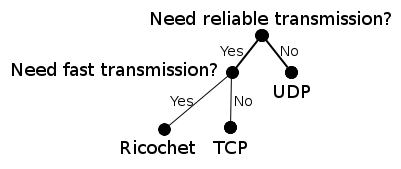
\includegraphics[height=1.5in, width=3in]{DecisionTree.png}
%%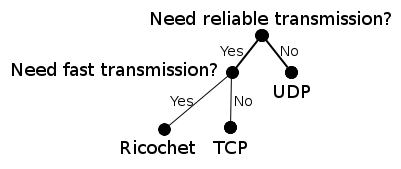
\epsfig{file=DecisionTree.png, height=1.5in, width=3in} -- ACM
%%\includegraphics{fly.pdf, height=1in, width=1in}
%%	\includegraphics{ClassificationTable.pdf}
%%        \vspace{-0.1in}
	%\caption{\bf Decision Tree Example}
	%\label{Fig:DT}
%\end{figure}

%From ARM 2009 paper:
%The first learning technique investigated is a decision tree (DT).
%This algorithm attempts to create a tree where a set of decisions
%leads down to a leaf node that can accurately classify a new example. A DT will attempt to produce the shortest and smallest tree
%possible while maintaining accuracy by looking for features that
%best split the data as completely as possible and use them closer to
%the root. DTs are designed for data sets with more than a binary set
%of classes, i.e., where there are more than two possible classifications of an appropriate transport protocol and parameter settings.

% Short on space and this was Erik's write-up. It should be redone.
%$\bullet$ {\bf Random Decision Forests.}
%Random Decision Forests are a composition of decision trees where key aspects of each tree's functionality include some form of randomness. The random elements will create differing trees resulting in different paths to arrive at a classification.
%After the forest is created, each tree will give a classification for the input data. The forest will select the most common classification returned by the composition of trees~\cite{Lin:06}.
%
%There are several strategies to introducing the randomness in a Random Forest. One strategy is to select random best-split characteristics attributes from the input data~\cite{Breiman:01}. The second method strategy is to randomly select which best-split features the tree will split on~\cite{Dietterich:2000}. A third method randomly selects subsets of the input data to achieve 100\% accuracy in classification on training data and increased accuracy in classification of unknown data~\cite{Ho:98}.
%Lin and Yongho~\cite{Lin:06} also mention a fourth method called Extreme Randomness which combines the randomness in attribute selection and in splitting features.

$\bullet$ {\bf Support Vector Machines.}
Support Vector machines (SVMs) are designed to find the greatest equal divide between classification axes for groups of input data. The SVM uses training data to build a model of data classification and obtain the greatest divide~\cite{Hoffert:10}. The training values are flagged with a classification schema so that when new data points are entered the SVM will use the separation to determine which schema-classification is appropriate for the new point. Finding the greatest separation will result in increased accuracy in classification for unknown input data.

	Fig.~\ref{Fig:SVM} shows group 1 (denoted by filled circles), group 2 (denoted by open circles), and an unknown input in gray. The circles in black are training examples, and the solid line is the greatest separation between the groups that the SVM will use to classify to which group the new entry belongs. An SVM would select the solid line for classification which maximizes the likelihood of appropriate classification for any new data. The dashed line represents a possible classification that accurately separates the existing data. When new data becomes available (as denoted by the gray circle) the SVM would have the highest likelihood of correct classification and would classify the gray circle into group two.

\begin{figure}[t]
	\centering
	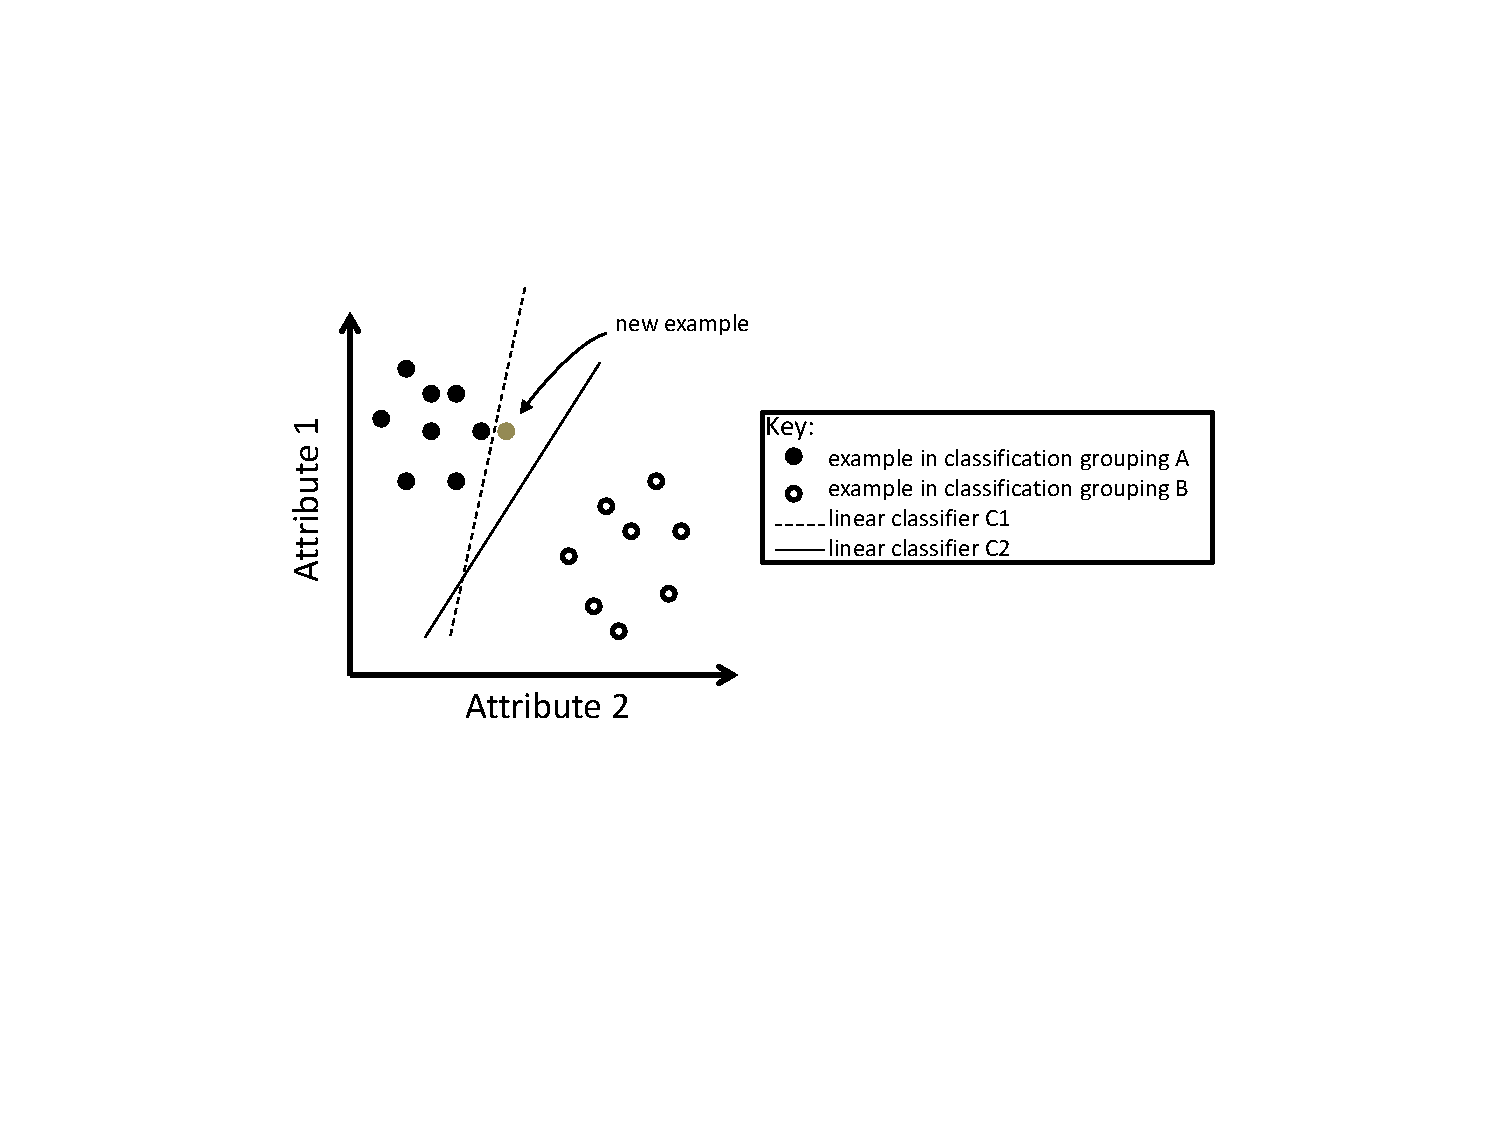
\includegraphics[height=1.5in, width=3in]{SVM.pdf}
%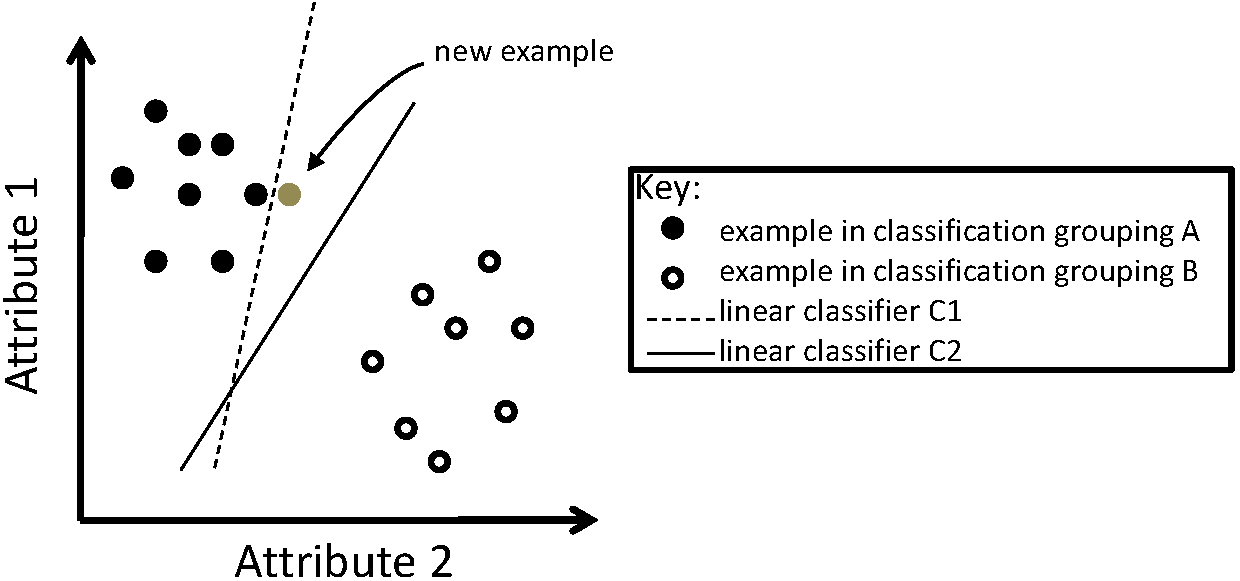
\epsfig{file=SVM.png, height=1.5in, width=3in}
%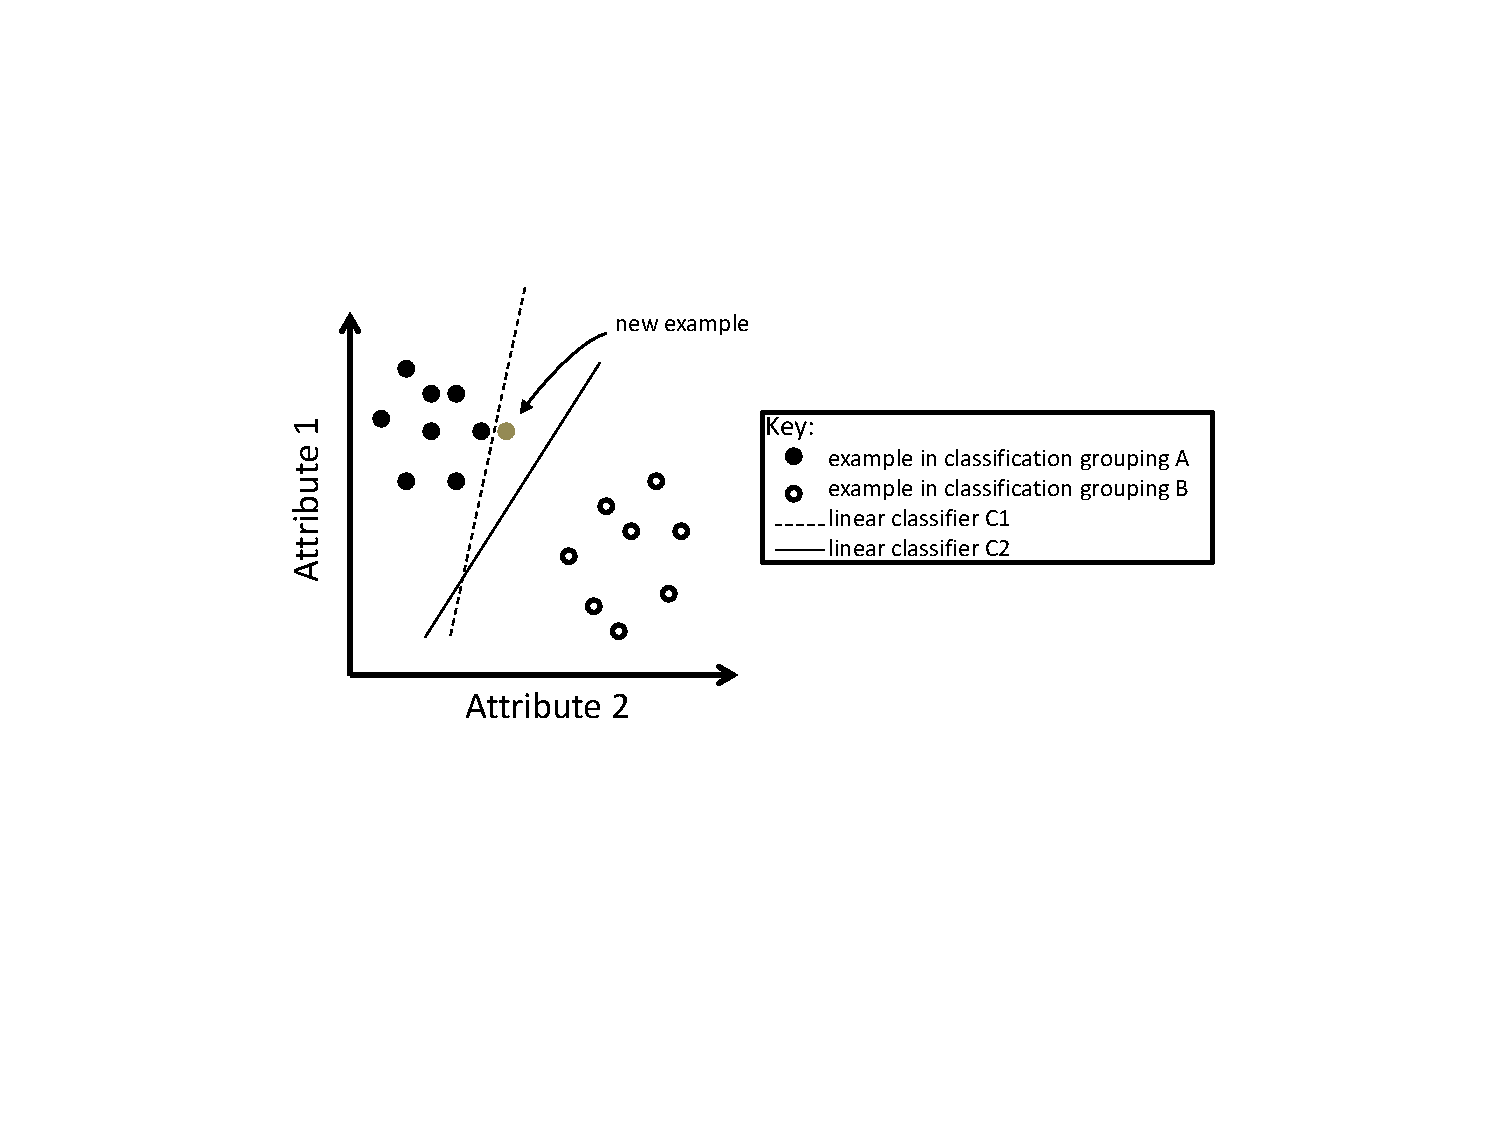
\epsfig{file=SVM.pdf, height=1.5in, width=3in} -- ACM
%\includegraphics{fly.pdf, height=1in, width=1in}
%	\includegraphics{ClassificationTable.pdf}
%        \vspace{-0.1in}
	\caption{\bf Support Vector Machine Example}
	\label{Fig:SVM}
\end{figure}

	%When points of differing flag characteristics become centrally located, mathematical transformation [Would I need a Source for this? it is a common mathematical practice] into hyper-planes allow the SVM to make the proper classification. The timeliness of which the SVM responds is dependant on the Kernel it uses~\cite{Hoffert:11}.

%Support Vector machines utilize input attributes, such as 'x' and 'y' values, to plot where the input data lies on a plane. The input values are typically flagged to be a negative data point, a positive data point, or some other classification schema. The machine then calculates a vector distance to each point on the plane from the origin. Predefined ranges of distance will determine which decision the Machine will make in classifying a data point as positive or negative. When points of differing flag characteristics become centrally located, mathematical transformation
%
 %[SOURCE] \emph{\textbf{Erik, is this a reminder to add a source for this statement? If so, please send me a citation when you have one ready.}}
%
%formulas are used to bring in additional mathematical dimensions to allow the SVM to make the proper classification. The calculation times for the SVM is dependent upon the kernel being used (\emph{e.g.}, linear, polynomial, radial basis function)~\cite{Hoffert:11}.
%
%
%From NPA Journal Article, page 9:
%``SVMs are supervised learning methods used for classification and prediction. Given a set
%of training examples where each example is denoted as belonging to a particular class or grouping, an SVM builds a model that predicts into which grouping a new example should be
%categorized. The SVM generates the boundaries between the different groupings to maximize
%the differences between the groupings. This maximization helps
%to correctly classify new
%examples that have not been used in training the SVM model using the heuristic of locality, \emph{i.e.}, examples that belong in the same group should be fairly close to each other in the classification space.
%Fig. 3
%illustrates
%conceptually how an SVM makes its determination for classification
%boundaries. The examples in grouping A are represented by solid circles while the examples
%in grouping B are represented by hollow circles. For simplicity and clarity, the examples are
%classified using two attributes. The dashed line C1 and the solid line C2 represent two different classifiers. An SVM produces a classifier similar to C2 since i
%ts margin between the two
%classification groupings is larger than with C1. A new example (\emph{i.e.}, a solid grey circle) that
%needs to be classified using the SVM belongs in classification grouping A. The example is close to the line C1 but on the opposite
%side of the rest of the examples for that grouping and
%is therefore incorrectly classified whereas with C2 the new example would be correctly classified. An SVM maximizes the margin of differences between classification groupings. [Can add figure]''

$\bullet$ {\bf Artificial Neural Networks.}
The artificial neural network (ANN) is an AI technique based on a biological model
of the human brain. An ANN has the useful ability to find patterns in empirical data
to generalize its behavior to similar, but not previously encountered, data. [1] Each
node in the network, called a \emph{neuron}, outputs a nonlinear transformation of a weighted
sum of its inputs --- that is, \emph{f}($\sum$$w_i$$x_i$) for some function \emph{f}
(known as the activation function), inputs $x_i$, and associated weights $w_i$.

These neurons are
typically arranged in discrete layers, namely the input layer, zero or more hidden
layers, and the output layer. Nodes in the input layer receive data from the
environment, and nodes in the output layer produce the network's learned response to
the given input. The hidden layers lie between the input and output layers and are
``hidden'' in that their states cannot be known based on the input and output alone. In
general, each layer produces input for the neurons in the next layer, although some
networks' structures (called recurrent)~\cite{Philips-Wren:12} send some output from one layer to an earlier layer or to nodes
in the same layer.

% Jeremy, in general the BN stuff needs to be shortened quite a bit. The general description in this section should be comparable in length to other AI techniques (i.e., about 1/4 page).
$\bullet$ {\bf Bayesian Networks.} A Bayesian network is a structured representation of the attributes of a system and their interconnected probabilities which represent the system as a coherent whole~\cite{Darwiche:10}.
%A Bayesian network is a way of structuring
%probabilistic information about a situation into a coherent whole.~\cite{Darwiche:10}
The network establishes this structure  by linking its nodes together in a directed acyclic graph of causal relationships, where for nodes \emph{A} and \emph{B}, \emph{A} $\rightarrow$ \emph{B} means that the value of node \emph{A} is one cause of the value of node \emph{B}. (Technically, the direction of causality is not always important because of the nature of probabilities. Knowing that the effect happened makes it more likely that the cause also happened, just as knowing that the cause happened makes the effect more likely.) This  structure can then be used to infer the most likely state of  any given node given the state of any or all of the other  nodes in the network. For instance, if \emph{A} represents contact  with a diseased person and \emph{B} represents contraction of the  disease, \emph{A} causes \emph{B}, and there is some probability, written as \emph{Pr}(\emph{B}|\emph{A}), that, given that \emph{A} occurs, \emph{B} also occurs. This probability is stored in the Bayesian network in the data structure for node \emph{B}, and the probability of \emph{A} occurring in the first place, \emph{Pr}(\emph{A}), is stored in node \emph{A}.

%The network establishes this structure by linking its nodes together in causal relationships, where for nodes A and B, A $\rightarrow$ B means that the value of node A is one cause of the value of node B. This structure can then be used to infer the most likely state of any given node given the states of any or all of the other nodes in the network.

In general, each node has an associated probability table that lists the probability of each of its possible values given every possible combination of its causes' values. If memory resources are scarce, the probability of the last possible value  can be omitted since it can be calculated. For example, in the network shown in Figure~\ref{Fig:BayesianNet}, where each variable can be  either true or false, node \emph{C}'s probability table contains four  rows, with the understanding that the four probabilities that \emph{C} is false are easily calculable from the probabilities that \emph{C} is true. Likewise, node \emph{D}'s probability table is also listed based on the value of node \emph{C}.

\begin{figure}[t]
	\centering
	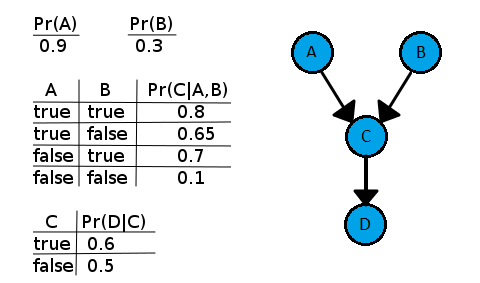
\includegraphics[height=1.5in, width=2.5in]{BayesianNetwork.png}
% 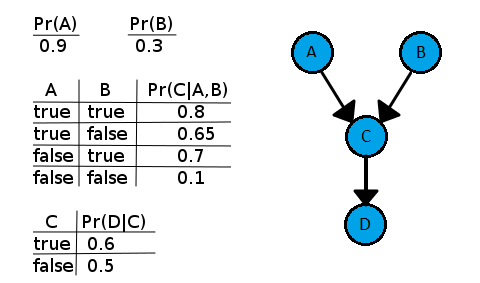
\epsfig{file=BayesianNetwork.png, height=1.5in, width=2.5in} -- ACM
%\includegraphics{fly.pdf, height=1in, width=1in}
%	\includegraphics{ClassificationTable.pdf}
%        \vspace{-0.1in}
	\caption{\bf Bayesian Network Example}
	\label{Fig:BayesianNet}
\end{figure}

One key concept of Bayesian networks is that of blocking nodes --- nodes that, when their values are known, make the values of certain other nodes independent of each other. For instance, in Figure~\ref{Fig:BayesianNet}, the value of \emph{D} is influenced by \emph{C} and therefore by \emph{A} and \emph{B}, unless the value of \emph{C} is already known. In that case, \emph{D} becomes independent of \emph{A} and \emph{B} because \emph{C} blocks the paths from \emph{A} to \emph{D} and from \emph{B} to \emph{D}. Knowledge of the conditional independences between nodes can simplify the algorithms that work with a given Bayesian network and improve their performance by pointing out which nodes can be ignored.

%This structure can then be used to infer the state of any given node given the states of any or all of the other nodes in the network. One key concept of Bayesian networks is that of blocking nodes --- nodes that, when their values are known, make the values of certain other nodes independent of each other. For instance, in the example with A $\rightarrow$ B $\leftarrow$ C, the value of A is influenced by B and therefore by C, unless the value of B is already known. In that case, A becomes independent of C because B blocks the path from C to A.
%Knowledge of the conditional independencies between nodes can simplify the algorithms that work with a given Bayesian network and improve their performance by pointing out which nodes can be ignored.

Because it is generally easier for a Bayesian network to  learn the appropriate values for its probability tables than  to learn the network topology, it is not uncommon to assume  some canonical network structure when learning Bayesian  networks from data, such as the particularly common \emph{na\"{i}ve Bayes}~\cite{Darwiche:10}.
In a na\"{i}ve Bayesian
network, there is one node \emph{C}, typically referred to as the class variable,
and one or
more nodes \emph{A$_{i}$}, referred to as attributes,
such that \emph{C} $\rightarrow$ \emph{A$_{i}$}.

There are no direct associations between attributes, so every attribute is independent of all other attributes if the value of \emph{C} is known. For the problem of classification, such as when a system must select an appropriate transport protocol for a given quality of service (QoS), na\"{i}ve Bayesian networks produce surprisingly accurate results, considering that the attributes may not be independent in reality. In fact, this structure's predictive performance is on par with other classifiers such as 
C4.5.~\cite{Friedman:97}\cite{Quinlan:93}
If the network instead learns a \emph{tree-augmented} na\"{i}ve structure, in which the attributes are caused by other attributes in a tree structure in addition to being caused by the classifier, the network's accuracy consistently exceeds that of other classifiers and those of a na\"{i}ve Bayesian network.

%can be used for medical diagnosis of patients with certain symptoms. Medical experts are questioned \emph{a priori} regarding 

\section{Classification of AI Approaches}
\label{classification}
This section classifies or ``taxonomizes'' AI/ML approaches based on the needs of adaptive DRE systems as outlined in section ~\ref{taxonomy} as outlined in Table~\ref{tab:summary}. In particular, each AI approach surveyed is classified on the 4 properties needed for adaptive DRE systems, namely (1) supporting a distributed environment, (2) supporting real-time requirements, (3) supporting an embedded environment, and (4) incorporating new data into the approach as it becomes available while the system is running.

\begin{table*} % TODO: Make the font green for a checkmark and red for an X.
	\large
	\caption{Summary of AI/ML Techniques}
	\centering
	\begin{tabular}{c|c|c|c|c|c}
	AI/ML Method              & Distributed & Real-Time & Embedded & Robust & Autodidactic \\
	\hline
	Artificial Neural Network & \cmark      & \cmark    & \cmark   & \cmark & \xmark \\
	Bayesian Network (dynamic & \cmark      & \xmark    & \cmark   & \xmark & \xmark \\
	structure)                &             &           &          &        &        \\
	Bayesian Network (static  & \cmark      & \cmark    & \cmark   & \xmark & \bf{?} \\
	structure)                &             &           &          &        &        \\
	Expert System             & \cmark      & \xmark    & \xmark   & \xmark & \cmark \\
	Reinforcement Learning    & \cmark      & \xmark    & \cmark   & \xmark & \xmark \\
%	Decision Tree             & \cmark      & \cmark    & \cmark   & \xmark & \xmark \\
% Why did we not have a subsection of section 5 for decision trees?
% Jeremy, I'll work on decision trees and random forests after you make changes for Bayesian networks (i.e., save space).
	Random Forest             & \cmark      & \cmark    & \cmark   & \cmark & \xmark \\
	Support Vector Machine    & \cmark      & \cmark    & \cmark   & \cmark & \xmark
	\end{tabular}
	\label{tab:summary}
\end{table*}

%\begin{figure*}[t]
%	\centering
%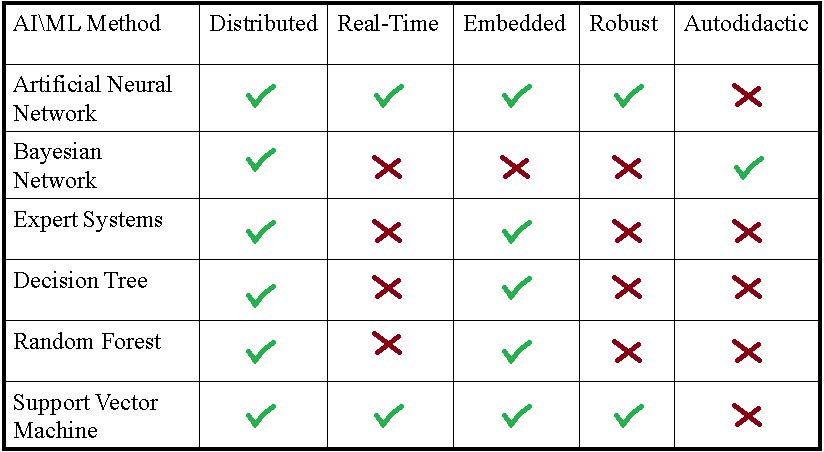
\epsfig{file=Table.jpg, height=3in, width=5.5in} -- ACM
%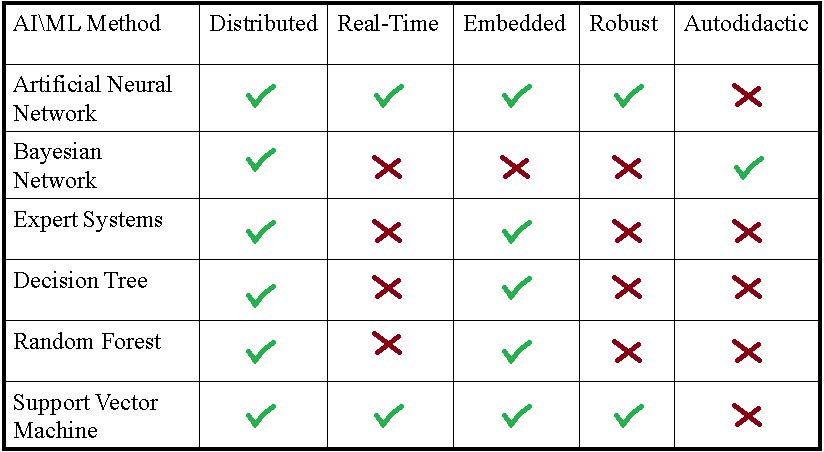
\includegraphics{Table.jpg, height=1in, width=1in}
%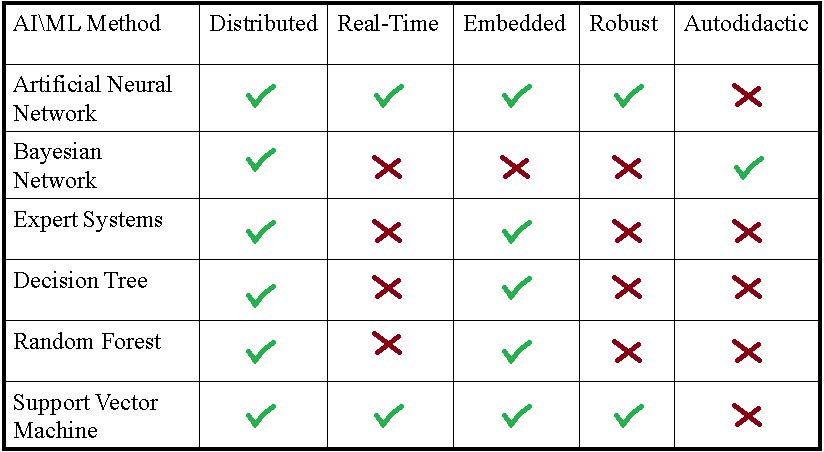
\includegraphics[height=3in, width=5.5in]{Table.jpg}
%	\includegraphics{ClassificationTable.pdf}
%        \vspace{-0.1in}
%	\caption{\bf Classification Table}
%	\label{Fig:ClassTable}
%\end{figure*}

$\bullet$ {\bf Artificial Neural Networks.}
An ANN is generally a  good fit for an adaptive DRE system, but it suffers from difficulty with learning over time.

\emph{Distributed.} After training, an ANN's output is deterministic as it depends only on the input, the network's static structure, the weights that have been learned, and the neurons' activation functions. Thus, identical ANNs distributed across a DRE system will all reach the same conclusion given the same input.

\emph{Real-time.} An ANN is ideal for a real-time system because the time it  takes to process any set of input data is bounded by the number of connections between the neurons, and that number  is known at compile-time. As a result, the computation time of a given ANN is constant.

\emph{Embedded.} Because an ANN maps each set of inputs directly to a set of outputs, even for inputs that it has not yet encountered, it is ideal for making decisions without human intervention.

\emph{Robust to new inputs.} Regardless of the training set, an ANN can produce output for every input set. Moreover, it interpolates between the training outputs when used on inputs outside of the training set, which can improve accuracy if the output values can be placed in a meaningful order (\emph{e.g.} 0 to 5 or low, medium, and high). In general, an ANN can be used reliably  on both known and previously unencountered inputs for a classification given a set of attributes, such as the attributes that determine the communication protocol that should be used to maintain a given quality of service~\cite{Hoffert:10}.

\emph{Autodidactic.} Unfortunately, an ANN does not easily learn from experience. The correct output must be known before the ANN can learn from a mistake, which implies either a more accurate AI technique employed alongside the ANN, a problem whose solution always becomes obvious in retrospect, or human intervention; and then the ANN must be trained again on the entire training set in addition to the new information that it is to learn. This training may conceivably be done on a separate processor in order to preserve the real-time requirement for using the network, but the time required for training is unbounded. The training is, however, deterministic, which is amenable for adaptivity in a distributed system.

% Jeremy's previous write-up.
%An ANN is generally a good fit for an adaptive DRE system. It can be used reliably for classification of environmental properties to allow the system to adapt to changing conditions. [2] After training, an ANN's output is deterministic as it depends only on the input, the network's static structure, the weights that have been learned, and the neurons' activation functions. Thus, identical ANNs distributed across a DRE system will all reach the same conclusion given the same input.
%
%An ANN is ideal for a real-time system because the time it takes to process any set of input data is bounded by the number of connections between the neurons, and that number is known at compile-time. Moreover, an ANN’s training is deterministic, which is amenable for adaptivity in a distributed system. An ANN is also is capable of reaching a decision without the help of a human, which makes it compatible with an embedded system’s typical lack of user interaction.
%
	%Unfortunately, an ANN does not easily learn from experience. The correct output must be known before the ANN can learn from a mistake, which implies either a more accurate AI technique employed alongside the ANN or human intervention, and then it must be trained again on the entire training set in addition to the new information that it is to learn. This training may conceivably be done on a separate processor in order to preserve the real-time requirement for using the network, but the time required for training is unbounded.

% Jeremy, in general the BN stuff needs to be shortened quite a bit. The taxonomizing in this section should be comparable in length to other AI techniques (i.e., about 1/3 page).
$\bullet$ {\bf Bayesian Networks.}
The general definition of a Bayesian network offers few guarantees about its timeliness or how it can learn over time. In particular, some implementations learn by adding or removing nodes and changing the connections between them. \textbf{\emph{[citation needed]}} This learning method removes the bound on the time required to analyze the network, making it fail the Real-Time and Autodidactic requirements. To maximize its ability to address all of the needs of an adaptive DRE system, we assume for the rest of this section that a Bayesian network does not change its structure in either of these ways. Under this restriction, Bayesian networks address most of the properties of adaptive DRE systems fairly well but are lacking in some areas.

	\emph{Distributed.} A Bayesian network, although it deals with probabilities, is deterministic because it calculates the probabilities instead of the actual values of nodes, which allows every part of a distributed system working with the same network to reach the same conclusions.
	
	\emph{Real-time.} After a Bayesian network is constructed, every invocation on the network for adaptive guidance satisfies the timeliness requirement of a real-time system by being bounded by the number of nodes in the network and the number of connections between them. The fact that the network is acyclic guarantees that no edge can be used more than once and that probabilities for each node's values do not need to be recalculated during the same invocation (\emph{i.e.}, a node cannot be a direct or indirect cause of itself, so it cannot affect its own probabilities). Some invocations might require fewer calculations because of conditional independence, but never more.
	
	\emph{Embedded.} Since a Bayesian network is used to determine the most likely value of a node given all available information, it can make decisions with high accuracy without human intervention, as embedded software systems require.
	
	\emph{Robust to new inputs.} A Bayesian network deals directly with probabilities, so it can be guaranteed to produce for any question the most likely answer given everything that it has learned. However, the opinion of a Bayesian network with discrete values for its nodes, which for the purposes of speedy computation and ease of understanding are usually used (with continuous variables being mapped to discrete variables through step functions~\cite{Friedman:96}), can be skewed by its lack of support for interpolation. For instance, if a Bayesian network is designed to classify a risk as either low or high, then it will never indicate any level of risk between those two extremes.
	
	\emph{Autodidactic.} Some Bayesian networks can learn at run-time easily and in bounded time by storing frequency counts, which can be used to calculate probabilities, rather than storing probabilities directly. 

% Jeremy, I've cut out the figure - there's one already for BNs (and we might want to cut that out later). Please revise (or even eliminate) the text below that references the 2nd BN figure.
For instance, a na\"{i}ve Bayesian network used to detect lies might be defined as in Figure~\ref{Fig:BayesianNetLying}, where \emph{C} represents the truth or falsehood of a statement, \emph{A} represents a contradiction with a previous statement, and \emph{B} represents whether the speaker's eyes are pointed down or not. \emph{Fr(C)}, where \emph{Fr} stands for frequency, is the number of times \emph{C} has occurred, and \emph{Fr(A|C)} is the number of times \emph{A} has occurred at the same time as \emph{C}.

For example, if the speaker makes a consistent statement with eyes forward, it will be classified, given the frequencies in the figure, as a true statement. If the statement is in fact true, then \emph{Fr(C = Truth)}, \emph{Fr(A = Consistent $|$ C = Truth)}, and \emph{Fr(B = Eyes Forward $|$ C = Truth)} can all be incremented to reinforce this behavior. If the statement is not true, then the corresponding frequencies where \emph{C} $\neq$ \emph{Truth} can be incremented as negative reinforcement, making a classification of \emph{Truth} less likely by making \emph{Lie} more likely. Even if \emph{C} had more than two possible values, such as \emph{Truth}, \emph{Half-Truth}, and \emph{Lie}, negative reinforcement could be applied with the same rule.

Unfortunately, while this method clearly works for a na\"{i}ve Bayesian network such as the one in the figure, but the problem is not always so simple. Consider the network given by \emph{A} $\rightarrow$ \emph{B} $\rightarrow$ \emph{C}. If, for instance, the values of \emph{A} and \emph{C} can be measured but that of \emph{B} cannot, then frequencies related to \emph{B} must be changed without being certain of its value. The most obvious way to handle this situation is to update each applicable frequency for \emph{B} (\emph{i.e.}, \emph{Fr}(\emph{B} $|$ \emph{A}) and \emph{Fr}(\emph{C} $|$ \emph{B}) for every possible value of \emph{B} and the measured values of \emph{A} and \emph{C}). However, more research is required in order to determine whether this method is mathematically sound and whether it works correctly for every Bayesian network with a static structure.

%\textbf{\emph{I'll need to think about how this learning technique could be used in a network where C isn't the direct cause of everything, like A $\leftarrow$ C $\rightarrow$ B $\rightarrow$ D. How would the frequencies for D change after finding out whether C is right or wrong? My first thought is that whether B is right or wrong would also have to be determined, but can that always, or ever, be done? And then how would B's frequencies change: based on the accuracy of C or on the accuracy of B? For now, all I know for sure is that this technique should work for any na\"{i}ve Bayesian network.}}
%
%\textbf{\emph{Jeremy, we'll table my comment above for now. We can address it in a different venue later.}}

	The time required for learning at run-time is thus bounded by the number of nodes, the number of connections between the nodes, and the number of possible values for each node, all of which are known \emph{a priori}. A Bayesian network's learning as well as its predictions can fit the requirements of a DRE system in that this means of learning over time is deterministic (given a consistent means of determining whether a prediction was correct), operates in bounded time, and requires no human intervention. But in a network in which some nodes' actual values cannot always be measured in retrospect, this learning method has not been proven to produce correct results.

% Jeremy's previous taxonomization:
%Bayesian networks fit adaptive DRE systems fairly well. Adaptation is supported by the ability of certain types of Bayesian networks to place multiple attributes in the right class, which can be used to determine what adaptations should be made because of changes pertaining to the running of the system. In addition, Bayesian networks, although they deal with probabilities, are deterministic because they calculate the probabilities instead of the actual values of nodes, which allows every part of a distributed system working with the same network to reach the same conclusions.
%
%After a Bayesian network is constructed, every invocation on a Bayesian network for adaptive guidance satisfies the timeliness requirement of a real-time system by being bounded by the number of nodes in the network and the number of connections between them. Some invocations might require fewer calculations because of conditional independence, but never more. Also, since a Bayesian network is used to determine the most likely value of a node given all available information, it can make decisions with high accuracy without human intervention as embedded software systems require.

% Cut to save space
%\begin{figure}[t]
	%\centering
	%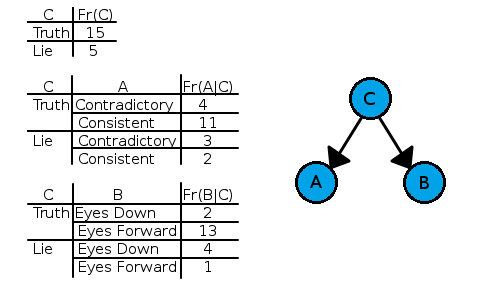
\includegraphics[height=1.5in, width=2.5in]{BayesianNetwork-LyingFrequencyCounts.png}
%%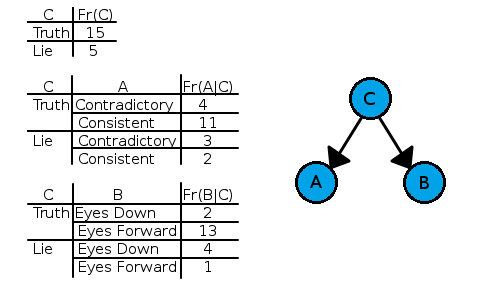
\epsfig{file=BayesianNetwork-LyingFrequencyCounts.png, height=1.5in, width=2.5in} -- ACM
%%\includegraphics{fly.pdf, height=1in, width=1in}
%%	\includegraphics{ClassificationTable.pdf}
%%        \vspace{-0.1in}
	%\caption{\bf Bayesian Network Example for Lying}
	%\label{Fig:BayesianNetLying}
%\end{figure}

%A Bayesian network can also learn at run-time easily and in bounded time by storing frequency counts, which can be used to calculate probabilities, rather than storing probabilities directly. For instance, a na\"{i}ve Bayesian network used to detect lies might be defined as in Figure~\ref{Fig:BayesianNetLying}, where \emph{C} represents the truth or falsehood of a statement, \emph{A} represents a contradiction with a previous statement, and \emph{B} represents whether the speaker's eyes are pointed down or not. \emph{Fr}(\emph{C}), where \emph{Fr} is short for frequency, is the number of times \emph{C} has occurred, and \emph{Fr}(\emph{A}|\emph{C}) is the number of times \emph{A} has occurred at the same time as \emph{C}.
%
%For example, if the speaker makes a consistent statement with eyes forward, it will be classified, given the frequencies in the figure, as a true statement. If the statement is in fact true, then \emph{Fr}(\emph{C} = Truth), \emph{Fr}(\emph{A} = Consistent | \emph{C} = Truth), and \emph{Fr}(\emph{B} = Eyes Forward | \emph{C} = Truth) can all be incremented to reinforce this behavior. If the statement is not true, then the corresponding frequencies where C $\neq$ Truth can be incremented as negative reinforcement, making a classification of Truth less likely by making Lie more likely.
%
%Even if C had more than two possible values, such as Truth, Half-Truth, and Lie, negative reinforcement could be applied with the same rule. The time required for learning at run-time is thus bounded by the number of nodes, the number of connections between the nodes, and the number of possible values for each node, all of which are determined before deployment. A Bayesian network's learning as well as its predictions can fit the requirements of a DRE system in that this means of learning over time is deterministic (given a consistent means of determining whether a prediction was correct), operates in bounded time, and requires no human intervention.

$\bullet$ {\bf Expert Systems.} While expert systems support some of the properties for adaptive DRE systems, multiple factors make expert systems less than ideal approaches in these contexts.

\emph{Distributed.} Expert systems are approprite for use in distributed environments since the results of using an expert system are deterministic. Expert systems with identical facts, rules, and inference engines can be deployed on computing nodes in the distributed system so that all nodes will generate the same advice. 

\emph{Real-time.} Expert systems typically utilize facts, rules, and an inference engine to provide solutions to problems based on human experts. The inference engine uses the facts and rules to infer knowledge which can also create new facts and initiate the use of additional rules. The inference engines creates this lattice or web of information that interconnects rules and facts and changes dynamically.

However, the selection of relevant rules and facts within the inference engine depends upon the problem being addressed. Some rules and facts will not apply for particular problems. Accordingly, searching the rules and facts is not optimized for a given situation and the time complexity is unbounded.

\emph{Embedded.} Expert systems are typically used for decision support and provide guidance for human operators rather than being autonomous and implementing the advice given. This property makes expert systems not well suited for embedded environments.

\emph{Robust to new inputs.} Expert systems do not support interpolation or extrapolation of results. Inferences are made from the facts and the rules. However, unless adaptation decisions involve specific facts and rules an expert system will not be able to provide suitable guidance. Therefore, an expert system is not robust to handling inputs not previously encountered.

\emph{Autodidactic.} Since expert systems are based on facts and rules they are amenable to adding new facts and rules as they become available. Adding a rule or fact for the inference engine is straightforward (\emph{e.g.}, stating a fact for a Prolog knowledge base) and can be done in constant time. The inference engine will utilize any new fact or rule as soon as it has been added. However, as noted previously, the generation of inferences can have unbounded time complexity.

%Do we need to concern ourselves with the time complexity of adding a fact or rule? Or are we concerned with ease of use for the developer to incorporate new knowledge/data?

$\bullet$ {\bf Reinforcement Learning.} While reinforcement learning has good properties in general of exploring a solution space, its utilization of pseudo-randomness and probabilities makes it ill-suited for adaptive DRE systems.

\emph{Distributed.} Reinforcement learning can be distributed across nodes in a distributed system. However, a key aspect of reinforcement learning is the use of stochastic or probabilistic transitions. To reach a consensus where pseudo-randomness is not consistent across nodes would require a consensus protocol such as that outlined in the Byzantine Generals Problem~\cite{Lamport:82}. To address this problem each node could use the same seed(s) to generate pseudo-random values so that each node will make the same transitions at the same time.

\emph{Real-time.} Due to using probabilities in transition functions, the time complexity of reinforcement learning is unbounded. Potentially, there are cycles in the possible transitions so that transitions could traverse cycles an unbounded number of times. Therefore, reinforcement learning does not satisfy the bounded timeliness property of DRE systems.

\emph{Embedded.} When developing reinforcement learning, feedback is needed to determine ultimate success or failure. However, after reinforcement learning has been adequately trained, there is no intervention needed and the reinforcement learning can be used without human intervention.

\emph{Robust to new inputs.} Reinforcement learning is designed to determine a path (via transitions) from a start state to an end goal. If the goal is changed (via new inputs) then reinforcement learning will need to relearn its transitions. If the goals changes then the reinforcement learning needs to change as well. Therefore, reinforcement learning is not robust to new inputs.

\emph{Autodidactic.} As noted previously, the learning time for reinforcement learning is unbounded. Therefore, reinforcement learning does not fulfill the autodidactic property for adaptive DRE systems.


$\bullet$ {\bf Random Forests.}
Random Forests can be adapted to fulfill most of the requirements of a DRE system.

\emph{Distributed.} There are two possible ways of achieving determinism in a Random Forest. While pseudo-randomness is used to determine the trees in the forest, this pseudo-randomness can be limited to each node in the distributed system. The same pseduo-random value can be deterministically achieved using the same seed on each node. Alternatively, if the pseudo-randomness is non-deterministic (\emph{i.e.}, each node potentially uses a different seed) across all nodes, then consensus needs to be reached across the nodes using a protocol similar to the one outlined in the Byzantine's General Problem~\cite{Lamport:82}. The latter solution provides unbounded time complexity due to the potentially unbounded number of trees and tree depth. Therefore, Random Forests should limit pseudo-randonmess to within a node and not across nodes.

\emph{Real-time.} The timeliness of the Random Forest is dependent on the average depth \emph{n} of the trees and the number of trees \emph{m} in the forest, \emph{i.e.}, O(\emph{m} log \emph{n})\cite{Lin:06}. It is possible to bound time complexity further with depth limitations, tree pruning, and the complex method of feature splitting\cite{Ho:95} to address timeliness concerns. However, this bounding has implications for accuracy.

\emph{Embedded.} Random Forests are decision making systems capable of reaching a classification without the interaction of a human, fulfilling the requirement of embedded systems.

\emph{Robust to new inputs.} The Random Forests' ability to generalize is determined by the number of trees in the forest. As the number of trees increases, the generalization increases as long as each new tree is sufficiently different from all the other trees in the forest~\cite{Ho:95}.

\emph{Autodidactic.} For a Random Forest to incorporate new data, new classification trees of non-predetermined depth must be added to the forest [Ho, 2006]. Time complexity will become unbounded without depth limitations, limitations on the number of trees in the forest, and tree pruning. If the forest is limited in either the number of trees that can be added or the depth and breadth of each individual tree (which is needed to address timeliness concerns), accuracy can be lost. Therefore, Random Forests do not address the autodidactic needs of adaptive DRE systems. 

$\bullet$ {\bf Support Vector Machines (SVMs).} SVMs generally useful for adaptive DRE systems. They are particularly useful for processing inputs at runtime that have never been seen before, which emphasizes their adaptability and accuracy under such conditions~\cite{Hoffert:11}.

\emph{Distributed.} SVMs are ideal for distribution due to the deterministic nature of their decision making process.

\emph{Real-time.} Training of an SVM is unbounded. However, after the initial training is completed SVMs classify in constant time.

\emph{Embedded.} SVMs are decision making systems --- their classifications are done without the aid of human intervention allowing them to be implemented in an embedded system.

\emph{Robust to new inputs.} SVMs support classification for new inputs. Moreover, in certain situations the accuracy of an SVM w.r.t. new  inputs has been shown to be better than other AI/ML methodologies such as artificial neural networks~\cite{Hoffert:11}.

\emph{Autodidactic.} In order for an SVM to incorporate new classifications into the training set the SVM would have to be retrained. While an SVM is robust to data not included in training, the accuracy of an SVM is limited if it is not retrained with the new data. With an unbounded time complexity for training, SVMs do not support the autodidactic property.

\section{Analyzing Gaps}
\label{gap-analysis}
Per analysis of the AI techniques for adaptive DRE systems, no single technique addresses all five areas of concern. Additionally, there is no AI technique that sufficiently addresses the autodidactic property of adaptive DRE systems. Additional research of AI techniques is needed to better understand the challenges and trade-offs and to address these deficiencies to more fully support adaptive DRE systems.
%\textbf{\emph{One gap we can put here is being able to handle all the requirements for adaptive DRE systems. There doesn't seem to be any approach that handles all four concerns for adaptive DRE systems. For instance, some approaches can be updated while the system is running (\emph{e.g.}, expert systems can handle adding another rule). However, these systems aren't suitable for adaptive DRE systems (in the case of expert systems, there are timeliness concerns).}}

%\section{Concluding Remarks} -- REMOVE FOR SPACE
%\label{summary}
%DRE systems are being used for control in many important domains (\emph{e.g.}, power grid, shipboard computing environments, manufacturing). Historically, these systems have been analyzed a priori to provide for provisioning resources and determining behavior. However, these systems can benefit from adaptation to leverage resources more appropriately and to respond to environments or situations not encountered previously. Artificial intelligence approaches can be used to enable this type of adaptation.
%
%Many AI approaches have been developed over the years. Some of these approaches are more amenable than others relative to the properties and requirements of DRE systems. The work outlined in this paper has furthered this research in the following ways. The properties of DRE systems relative to adaptation have been clearly enumerated and defined. Several AI approaches have been summarized and taxonomized using the enumerated properties. Gap analysis has been performed to show areas of further investigation and research.
%
%The AI approaches included in this work are non-exhaustive. In particular, there are hybrid approaches that include aspects of multiple traditional AI approaches (\emph{e.g.}, neural networks and expert systems~\cite{Sahin:2012}). However, the taxonomy developed can be used to evaluate new or hybrid approaches for consideration with adaptive DRE systems.

%Our findings reflect two primary problems with existing work.  The first problem
%is a lack of existing support.  Several projects fill some of the gaps we have identified, but no project
%fills all the gaps.  Moreover, most projects are not actively maintained.
%In order for progress to be made in the area of adaptive
%networking, it is important that the development of software keep pace with the
%growth of the industry at large.
%
%Secondly, the existence of a standard would be greatly beneficial to expanding
%work on adaptive networking software, especially within specific network layers.
%Currently, projects pursue their goals by whatever method those involved
%perceive to be the best.  This allows for relatively quick progress to be made,
%but inhibits integration of elements from multiple different projects.  This
%shortcoming will become more pronounced as relevant software and concepts
%appear.  Hence, the lack of standards in this area is a major hurdle standing
%in the way of commercialized adaptive networking.
%
%Overall, we found several pieces of work related to protocol frameworks.  These
%ranged from specific protocol implementations to overhauls of the entire
%network stack.  Our taxonomy identifies some strengths of existing work, including
%support for non-standard protocols.
%However, we also reveal several important but absent features and areas for future
%work, most notably a lack of fine grained control over transitions from one
%protocol to another.

%\section*{Acknowledgments}
% 

{
\bibliographystyle{plain}
\bibliography{Survey}  % append .bib to the name for bibliography file
}

\end{document}